% Gerado automaticamente. No preambulo do documento use:
% \usepackage{pgfplots}
% \pgfplotsset{compat=1.18}
\definecolor{plotblue}{HTML}{2563EB}
\definecolor{plotorange}{HTML}{D97706}
\definecolor{plotgreen}{HTML}{059669}
\definecolor{plotpurple}{HTML}{7C3AED}
\definecolor{plotgray}{HTML}{374151}
\definecolor{plotred}{HTML}{DC2626}
\definecolor{plotteal}{HTML}{0F766E}
\definecolor{plotslate}{HTML}{64748B}

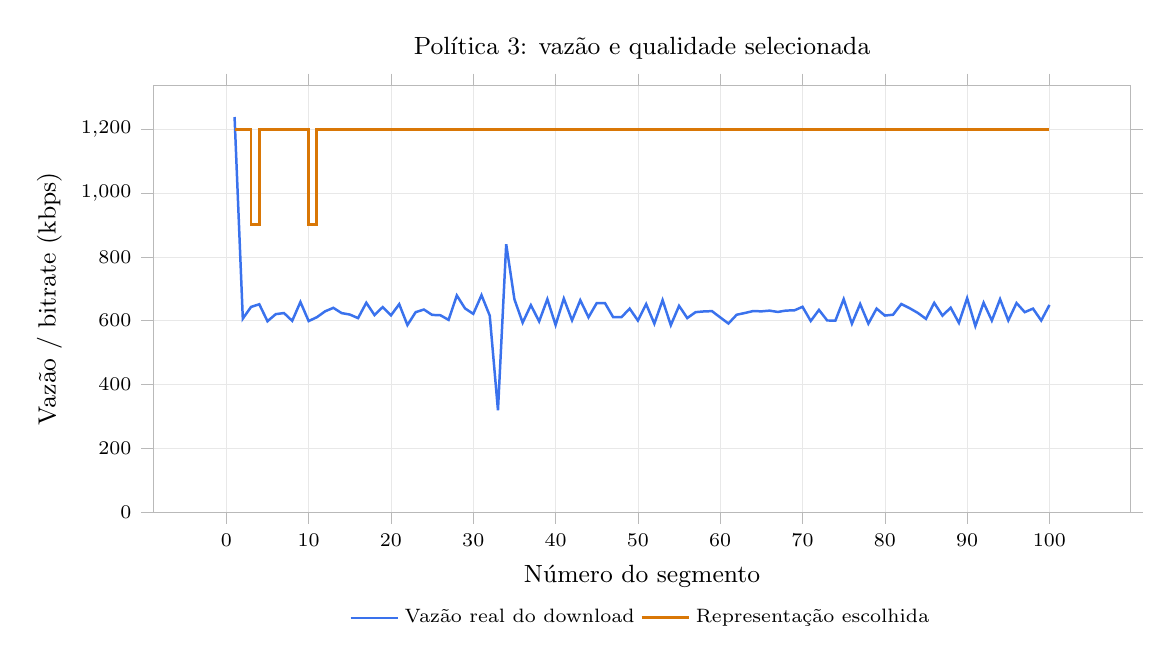
\begin{tikzpicture}
\begin{axis}[
    title={Política 3: vazão e qualidade selecionada},
    xlabel={Número do segmento},
    ylabel={Vazão / bitrate (kbps)},
    width=14cm,
    height=7cm,
    grid=major,
    grid style={line width=.12pt, draw=gray!18},
    axis line style={draw=gray!55},
    tick style={draw=gray!55},
    tick align=outside,
    title style={font=\small},
    label style={font=\small},
    tick label style={font=\scriptsize},
    legend cell align={left},
    legend style={at={(0.5,-0.20)}, anchor=north, legend columns=3, draw=none, font=\scriptsize},
    ymin=0,
    ymax=1337.37
]
\addplot+[plotblue, line width=0.9pt, mark=none, opacity=0.9] coordinates {
(1,1238.31)
(2,606.31)
(3,643.05)
(4,651.44)
(5,598.12)
(6,620.36)
(7,623.82)
(8,599.42)
(9,658.41)
(10,598.63)
(11,610.83)
(12,629.25)
(13,640.16)
(14,623.74)
(15,619.19)
(16,607.86)
(17,656.04)
(18,617.51)
(19,642.64)
(20,616.5)
(21,651.64)
(22,586.17)
(23,626.61)
(24,634.86)
(25,618.02)
(26,616.95)
(27,602.48)
(28,679)
(29,638.26)
(30,621.3)
(31,679.84)
(32,615.83)
(33,319.21)
(34,839.59)
(35,666.84)
(36,593.84)
(37,648.65)
(38,597.57)
(39,667.44)
(40,586.38)
(41,669.19)
(42,600.97)
(43,664.1)
(44,610.58)
(45,655.14)
(46,655.03)
(47,610.73)
(48,610.69)
(49,637.76)
(50,600.4)
(51,652.08)
(52,590.59)
(53,664.39)
(54,585.86)
(55,646.36)
(56,608.04)
(57,626.6)
(58,628.88)
(59,629.79)
(60,610.21)
(61,590.99)
(62,618.53)
(63,624.04)
(64,630.09)
(65,629.16)
(66,631.34)
(67,627.29)
(68,631.69)
(69,632.1)
(70,643.37)
(71,598.95)
(72,633.7)
(73,600.47)
(74,600.42)
(75,667.26)
(76,590.48)
(77,652.31)
(78,590.63)
(79,637.81)
(80,616.02)
(81,618.56)
(82,652.15)
(83,639.21)
(84,624.43)
(85,605.63)
(86,655.77)
(87,615.78)
(88,640.56)
(89,593.15)
(90,670.43)
(91,583.01)
(92,656.16)
(93,600.23)
(94,667.34)
(95,600.52)
(96,655.21)
(97,626.66)
(98,637.74)
(99,600.48)
(100,649.2)
};
\addlegendentry{Vazão real do download}
\addplot+[plotorange, const plot, line width=1.05pt, mark=none] coordinates {
(1,1200)
(2,1200)
(3,900)
(4,1200)
(5,1200)
(6,1200)
(7,1200)
(8,1200)
(9,1200)
(10,900)
(11,1200)
(12,1200)
(13,1200)
(14,1200)
(15,1200)
(16,1200)
(17,1200)
(18,1200)
(19,1200)
(20,1200)
(21,1200)
(22,1200)
(23,1200)
(24,1200)
(25,1200)
(26,1200)
(27,1200)
(28,1200)
(29,1200)
(30,1200)
(31,1200)
(32,1200)
(33,1200)
(34,1200)
(35,1200)
(36,1200)
(37,1200)
(38,1200)
(39,1200)
(40,1200)
(41,1200)
(42,1200)
(43,1200)
(44,1200)
(45,1200)
(46,1200)
(47,1200)
(48,1200)
(49,1200)
(50,1200)
(51,1200)
(52,1200)
(53,1200)
(54,1200)
(55,1200)
(56,1200)
(57,1200)
(58,1200)
(59,1200)
(60,1200)
(61,1200)
(62,1200)
(63,1200)
(64,1200)
(65,1200)
(66,1200)
(67,1200)
(68,1200)
(69,1200)
(70,1200)
(71,1200)
(72,1200)
(73,1200)
(74,1200)
(75,1200)
(76,1200)
(77,1200)
(78,1200)
(79,1200)
(80,1200)
(81,1200)
(82,1200)
(83,1200)
(84,1200)
(85,1200)
(86,1200)
(87,1200)
(88,1200)
(89,1200)
(90,1200)
(91,1200)
(92,1200)
(93,1200)
(94,1200)
(95,1200)
(96,1200)
(97,1200)
(98,1200)
(99,1200)
(100,1200)
};
\addlegendentry{Representação escolhida}
\end{axis}
\end{tikzpicture}
